%!TEX root=paper.tex

\section{Per-User Performance Monitoring}
\label{sec:user}

It is often the case that a service has diferent types of users: the paying and the free-for-evaluation ones, or the in-house and those in a different organization. 

In some other cases, it might be important for the maintainer of the API to understand the performance on a per-user basis, especially for situations where the system response time is a function of some individual user load\footnote{E.g. in GMail some users have a few dozen emails while other have tens of thousands: this difference in user loads will eventually induce a difference in the response times for different users}.

To support narrowing down the analysis to groups of users, or even individual users, the \tool must log together with every request grouping information for that request. The simplest way of achieving this is to take advantage of the architecture of Flask applications in which a global \code{flask.request} is used to retrieve session information which can in turn is normally used to identify the user sending the request. From the user one can obtain the group. 

The following code snippet shows how to configure the dashboard to enable user-by-user analysis\footnote{	If we wanted to group by the user group for example, the code would change slightly by replacing ``user.id'' with ``user.group.id''}: 

\begin{lstlisting}[style=custompython]  
# LOC #2: configure the dashboard
# to group requests by the user id
dashboard.config.group_by = 'User',
  lambda: Session.find(flask.request).user.id

\end{lstlisting}

The \code{dashboard.config.group\_by} is assigned a tuple with two elements, in which:  

\begin{itemize}
	\item \code{'User'} stands for the name of this particular grouping strategy
	\item \code{lambda: Session.find... } is a callback with no arguments, 
	that makes use of the global \code{flask.request} and extracts from 
	the request the current session, and in turn the user id\footnote{
		Note that every web service or application must have a way of 
		associating a request with a user. In fact, the Session.find(request) 
		was already an existing function in the analyzed system}
\end{itemize}

% \niceseparator

In Zeeguu, the \epFeedItems endpoint retrieves a list of recommended articles for a given user. As shown in \Fref{fig:ep}, this is the endpoint with the slowest response time and highest variability. The reason for this is that a user can be subscribed to anything from one to three dozen article sources and for each of the sources the system must compute the personalized difficulty of each article at every request. 


\begin{figure}[h!]
  \centering
  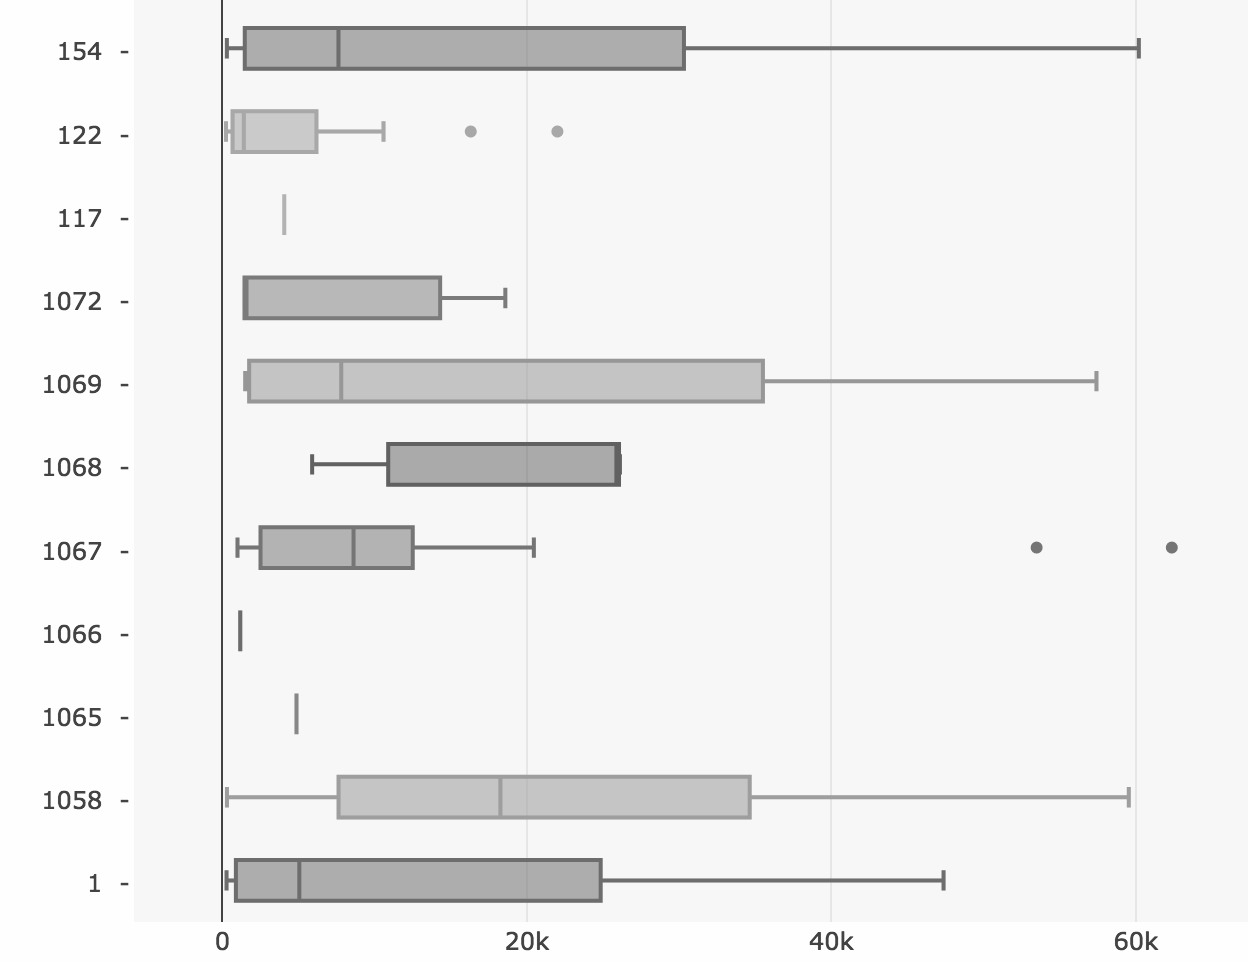
\includegraphics[width=.7\linewidth]{time_per_user}
  \caption{The \epFeedItems shows a very high variability across users}
  \label{fig:tpu}
\end{figure}


A \perspective{Per-User Performance} perspective should show the different response times for different users. \Fref{fig:tpu} presents a subset of the corresponding view in the \tool. The figure shows that the response times for this endpoint can vary considerably for different users with some extreme cases where a user has to wait a full minute until their recommended articles are shown\footnote{After seeing this perspective, the maintainer refactored the architecture of the system to move part the difficulty computation out of the interactive loop}.






